\chapter{Background}

\section{Heterogeneous Architectures}
\label{sec:heterogeneous}

Moore's law is an important concept for computer designers, specifying that the
number of transistors on a chip doubles approximately every second year. However,
as transistors are getting smaller, the amount of power they use have not been
decreasing at the same rate \cite{dark-silicon}.

This has led to an effect called dark silicon; it is simply not possible to
power all the transistors on a chip at the same time --- causing parts of
a chip to need to be turned off.

Heterogeneous architectures attempt to alleviate the dark silicon effect by
providing a number of different processing elements. These can be specialized for
doing special tasks by adding accelerators or implementing separate computing
elements for solving certain problems.

\subsection{The Single-ISA Heterogeneous MAny-core Computer}
\label{sec:shmac}
The Single-ISA Heterogeneous MAny-core Computer, SHMAC, is the Energy Efficient Computing Systems group
at the Norwegian University of Science and Technology's research project for investigating the
challenges and issues related to creating a heterogeneous computer architecture.

The architecture is tile-based, with a number of processing elements organized
in a grid and connected to their nearest neighbours. The tiles can be of varying
types, such as processor tiles or memory tiles. Processor tiles can contain
accelerators for accelerating various tasks, but all implement the same basic
ISA \cite{shmac-plan}.

%\subsection{Current Interconnect System in SHMAC}
%
%SHMAC implements a 2D mesh-based Network-on-a-Chip (NoC) interconnection network. 
%Currently, the system uses dimension-ordered (XY) routing, and store-and-forward
%switching with on/off flow control. The switching routine can be replaced in the
%future, should the current routine be found to cause performance bottlenecks \cite{shmac-plan}.
%
%\todo{Make sure the "goal"-part is valid}
%SHMAC does not implement DMA today, and data transfers are performed by the
%on-tile processors. A goal of this project is to explore the option of implementing
%a DMA module and testing it in a shared-bus system, before creating a prototype that
%can be implemented in SHMAC.

\section{The Bitcoin Currency}
\label{sec:bitcoins}
Bitcoin is a decentralized currency using a peer-to-peer network to replace
the financial institutions that are used to process transactions in conventional
currency systems.

The network keeps a ledger of all transactions in a linked list of blocks, called the
block-chain. Each block contains a list of all transactions executed since the last
block was published. Blocks are generated periodically through a process
called ``mining'', described in \ref{sec:bitcoin-mining}. This is due to the fact that
a valid block must satisfy the requirement that the hash of the block must be below a certain value
which is determined by a variable difficulty value used to limit the number
of blocks being generated each hour \cite{bitcoin}.

As an incentive to keep generating new blocks, a reward is offered on each new block
generated. This reward is currently at 25~bitcoins (467~USD as of the 9th of November, 2014)).
This reward is why bitcoin mining is a popular activity, and a reason for why
there are many initiatives to improve the performance of bitcoin mining systems.

\subsection{Mining Bitcoins}
\label{sec:bitcoin-mining}
The process of creating a new block in the bitcoin network is called ``mining''. The basic
principle of bitcoin mining is to create a block that generates a SHA-256 hash with
a value lower than a preset target value.

Since bitcoin mining is an NP-hard problem \cite{bitcoin-np}, the search for a valid block
hash has to be done by brute-force search. The block header contains several fields
that can be varied to produce different hashes, and it is also possible to include
or exclude transactions from the block in order to produce a hash with the desired
value.

Mining performance is measured in hashes per second, denoted H/s. Hashing is the
most computing intensive part of the algorithm for mining bitcoins, which is
why accelerating hashing is a priority.

\section{Cryptographic Hashing}

A cryptographic hash function, also commonly referred to as a digital signature or
a message digest, is a function that takes input data of varying size and
produces an output value of a constant size \cite{hashing-overview}.
% That article is a pain to read, it pains me to cite it

Cryptographic hash functions are designed to be one-way, meaning it should
not be computationally feasible to find the input data given the hash value,
and collision resistant, meaning that it should not be practical to find two
different sets of input data that produces the same output hash \cite{sha-spec}.

\subsection{The SHA-256 Hashing Algorithm}
\label{sec:hashing-algo}

The SHA-256 algorithm is a member of the set of algorithms referred to as the SHA-2 standard.
These are described in \cite{fips180-4} and consists of algorithms for producing hashes with lengths of 224, 256, 384 and 512 bits.
The algorithms use simple operations, limited to shifts, rotates, xor, and unsigned additions,
in addition to a lookup-table of constants, which allow for high-speed implementations in both
software and hardware. The different algorithms differ in how and with what parameters the various
operations are invoked.

SHA-256 is the algorithm used in cryptocoin mining. It operates on blocks of 512 bits
and keeps a 256-bit intermediate hash value as state.

Before the first block is processed, the initial hash value is set to a predefined
value. The entire message that is to be hashed is then padded by adding a 1 bit to
the end of the message and then appending zeroes until the length of the final block
is 448 bits. Then the length of the entire message, without padding, is added as a
64-bit big-endian integer to the end of the block.

Then, each input block is split into a 64 32-bit long expanded message block, where
each 32-bit word $W_j$ is defined according to the formula

\[ W_j = \left\{
	\begin{array}{l l}
		M_j & \quad j \in \left[0, 15\right]\\
		\sigma_1(W_{j - 2}) + W_{j - 7} + \sigma_0(W-{j - 15}) + W_{j - 15} & \quad j \in \left[16, 63\right]
	\end{array}
\right.\]

\noindent where $M_j$ is the $j$th word of the input message block and the functions
$\sigma_0$ and $\sigma_1$ are defined as

\[\sigma_0 = R^7(x) \oplus R^{18}(x) \oplus S^3(x)\]
\[\sigma_1 = R^{17}(x) \oplus R^{19}(x) \oplus S^{10}(x)\]

\noindent where the operator $R^n$ means right rotation by $n$ bits and $S^n$ means right shift by $n$
bits \footnote{Curiously, \cite{sha-spec} defines the operator $R$ as shift and $S$ as rotate.
We use the more intuitive definitions.}.

\subsubsection{The Compression Function}
\label{sec:sha-compr}
The compression function is the core of the SHA-256 algorithm. It uses a look-up table
of 64 constants, $K_j$, and the following functions when calculating the new intermediate
hash values:

\[Ch(x,y,z) = (x \wedge y) \oplus (\neg x \wedge z)\]
\[Maj(x, y, z) = (x \wedge y) \oplus (x \wedge z) \oplus (y \wedge z)\]
\[\Sigma_0(x) = R^2(x) \oplus R^{13}(x) \oplus R^{22}(x)\]
\[\Sigma_1(x) = R^6(x) \oplus R^{11}(x) \oplus R^{25}(x)\]

Before starting the iterations with the compression function, the intermediate
hash values from the previous message block are assigned to the variables $a$--$h$.

At the beginning of each iteration of the compression function, two temporary
values are calculated:

\[T_1 = h + \Sigma_1(e) + Ch(e, f, g) + K_j + W_j\]
\[T_2 = \Sigma_0(a) + Maj(a, b, c)\]

The new hash values are then assigned as follows:

\[\begin{array}{l}
	h \leftarrow g \\
	g \leftarrow f \\
	f \leftarrow e \\
	e \leftarrow d + T_1\\
	d \leftarrow c \\
	c \leftarrow b \\
	b \leftarrow a \\
	a \leftarrow T_1 + T_2 \\
\end{array}\]

The compression function is run 64 times, once for each extended message block word,
$W_j$. Afterwards, the intermediate hash for the message is updated by adding the
variables $a$--$h$ to the corresponding values of the intermediate hash values from
the previous message block.

When the final input block has been processed, the final hash is composed by
concatenating the intermediate hash values \cite{sha-spec}.

\section{Direct Memory Access (DMA)}

A DMA is used to offload the transfer of blocks of data between memory locations from
the processor(s) in a system. This allows the processors to work on other tasks or enter
a sleep state while data is being transferred.

In order for a hashing accelerator to be energy efficient and have better performance,
it is important that a processor does not have to do memory transfers by itself. Therefore,
a DMA module is being designed that can be used for transferring data to or from the hashing
module, and later be extended to work as a general DMA in the SHMAC architecture.

\subsection{The Purpose of DMA}

Without a DMA device, the CPU must do all data requested data transfers.
Processors would either have to rely on polling or interrupts \cite[p~589]{computer-construction}.
In polling, the processor checks the peripherals for requests, and in most cases the are no requests.
By using interrupts, one would spare the processor the inefficient amount of work done by polling, by letting interrupt signals into the CPU alert it for possible requests.
Nevertheless, in both cases the CPU still is responsible for data transfer itself.

% Devices do not directly ask the CPU to transfer data for them, they usually cause
% interrupts when something interesting has happened; it is then up to the CPU to
% take an action depending on what has happened. Such an action can for example be
% to transfer data to or from the peripheral. I think this should be clarified
% in the section above. -K.

% I mention "alert to possible request", does that satisfy?
% - T

Direct Memory Access was developed in order to relieve the CPU of this work \cite[p~592]{computer-construction}.
When a transfer request has been identified, the DMA module is activated by the CPU and provided with the necessary data for the task.
While the DMA transfers the data, the CPU is free to work on other tasks, or to go to idle mode.
When done with the transfer, the DMA module signals the CPU, and the CPU will handle the \todo{Hmmmm....}remaining work such as notifying requesting peripherals. How a DMA Engine should be implemented depends on the system environment.

DMA was also designed to perform data transfers with less overhead than on a CPU \cite[p~318]{encyclopedia}
A CPU is made for general-purpose work, and though the overheads depend on the CPU type, they include at least decrementing index and performing branching.
\todo{Concider removal}This can be avoided in a DMA module, as its \todo{This sounds cliche} hardware can be specifically designed to calculate addresses and counting down.

\subsection{Basic Requirements for DMA}
For data transfer, the minimum knowledge required is the address (source and destination), data register and a word counter \cite[p~876-877]{encyclopedia}.
A DMA module will require these to perform a data transfer.
Any other features may improve the DMA module in terms of additional functions, integration with the system, and efficiency, but without the these basic needs it cannot perform data transfer.

% \subsection{DMA Module Functionality}
% \todo{Documentation, documentation, documentation!}
% The minimum requirement of a DMA module is to be able to transfer data from one location to another.
% However, for an efficient implementation for a given system, there are several options to consider,
% such as operational modes, transfer types, integration with the rest of the system, and which
% registers and interrupts to provide. The architecture of the DMA module is affected by
% the options chosen, and how well they will fit in the SHMAC system.

\subsection{Operational Modes}
There are three operation modes defined for how the DMA will interact with the interconnect network:
\begin{description}
    \item[Burst mode.] \cite[p~876-877]{encyclopedia}
    The DMA has full ownership of the bus as long as the transfer is under execution.
    This is the fastest transfer mode for a DMA module, but it limits bus access for other
    peripherals as long as the DMA is executing the transfer.

    \item[Cycle stealing mode.] \cite[p~876-877]{encyclopedia}
    The DMA requests the bus as in burst mode, but relents control of the bus after transferring
    each byte of data. It will then re-request access to the bus for each transmission.
    In this way, the CPU and other peripherals can get earlier access to the bus if they need to.

    \item[Transparent mode.] \cite{dma-lecture}
    The DMA monitors the bus and transfers data only when the CPU or other modules are not performing operations that requires the bus.
    This is the slowest mode for the DMA itself, but also the one that allows the least slowdown for the CPU.
\end{description}

This is not really a property of the DMA Controller itself, but to the bus arbiter that handles bus requests on behalf of the DMA module.
The effect of this implementation may also differ between shared-media network and packet-switched network (such as in SHMAC).
The principles remain the same; how high priority should DMA transfers have, compared to other transfers in the system. 
Having transfers be as quick as possible, like in the burst mode, will make DMA transfers more efficient, but will also place the most restriction on the network for other modules and peripherals, should it occur at a time when many peripherals or tiles are attempting to perform data transfers.

A lower priority scheme will make data transfers go faster for other modules, but at
the same time, DMA transfers will be slower. Deciding the priority of a DMA transfer,
however, will be up to the routers in the network, \todo{True, but should this not be stated in the chapter where we explain our chosen designs?} and is therefore outside the scope of this project.

\subsection{Transfer types}
Transfer types \cite{microchip54} describes how the source and destination addresses are used in the transfer.
Some commonly used options are:
\begin{description}
    \item[Fixed-to-fixed transfers.]
    Both the source and destination addresses remain the same for each data transfer.
    This mode is suitable for transfers of single data between two fixed addresses,
    or if the DMA operates with single-word transfers.
    \item[Fixed-to-block transfers.]
    The source address is fixed, while the destination address increments.
    This is useful for storing data \emph{from} the buffer of, for instance, a serial
    communication peripheral, such as the 16C750 UART.
    It could also be used to do multiple copies of data from a single address to multiple addresses.
    \item[Block-to-block transfers.]
    Both source and destination addresses increment for each transfer.
    This is the scheme where entire blocks of data is transferred during a single operation.
    \todo{Perhaps mention this as a requirement?}
    \item[Block-to-fixed transfers.]
    The source address increments, while the destination address remains the same.
    This is useful when, for instance, transferring data \emph{into} the buffer of a
    serial communications peripheral.
\end{description}

More complicated DMAs also support \todo{Think it's mentioned in \cite{microchip54}, but it doesn't hurt to check} additional modes, such as using more complex patterns
when modifying the source and destination addresses or modifying the data in-flight.

\subsection{DMA Channel}
A DMA channel is defined \cite[p.~422]{DMAOxford} as an interface with own sets of registers.
Channels can be programmed to interface for selected peripherals in the system.
A channel is responsible for handling a requested data transfer, as it contains its own set of registers, used for controlling the operation and handling transfer addresses.
The appropriate number of channels depends on the system.
Microchip PIC24F \cite{microchip54} can have as many as 16 channels, while the Adapteva Epiphany \cite{epiphany} has 2 generic channel for each DMA module.

%\subsection{System and Data Registers}
%A DMA requires minimum a buffer for storing transfering data, as well as registers for load addresses and store addresses.
%At a minimum, a DMA requires registers containing the load and store addresses.
%Counters and a register for the maximum count is also needed when transferring blocks of data.
%\todo{What is a channel?}
%DMA modules often operate with multiple channels, each handling their own data transfers.
%A possible implementation for multiple channels is to have seperate registers for load addresses, store addresses and counts for each channel.
%Another possible implementation is to have a buffer for outgoing data, where request ID, load address and store address are combined in order to recognize the incomming data from the load memory and send them to the correct store address.
%In this case, one counter may operate with one load address and generate the requests at the time.
%
% - Commented out because I don't agree on this. -K.

\subsection{Word or byte addressing}
System memory is addressed either by word or by byte.
The DMA module used in the same system must follow the same type addressing.
A generic DMA module made for more than one system should offer the choice between word addressing or byte addressing, as part of the input configuration.

\subsection{DMA Integration Considerations regarding SHMAC}
\todo{Documentation, documentation, documentation... uhm... how do you document your separate ideas for the options?}

If the DMA module is to be integrated with SHMAC, there are some considerations that needs to be addressed.
The DMA module should be adapted to work as efficient as possible with SHMAC, and at the same time, it should also be possible to todo{Meh... sounds stupid. It's efficiency vs. generic that I'm trying to address} use it everywhere. 
A DMA module may be implemented as a separate shared DMA Controller tile in SHMAC, as seen in figure \ref{fig:DMATile}, or as an accelerator on an exisiting tile, for instance in a CPU tile, as seen in figure \ref{fig:DMAAccelerator}.

\begin{figure}[h!]
    \centering
    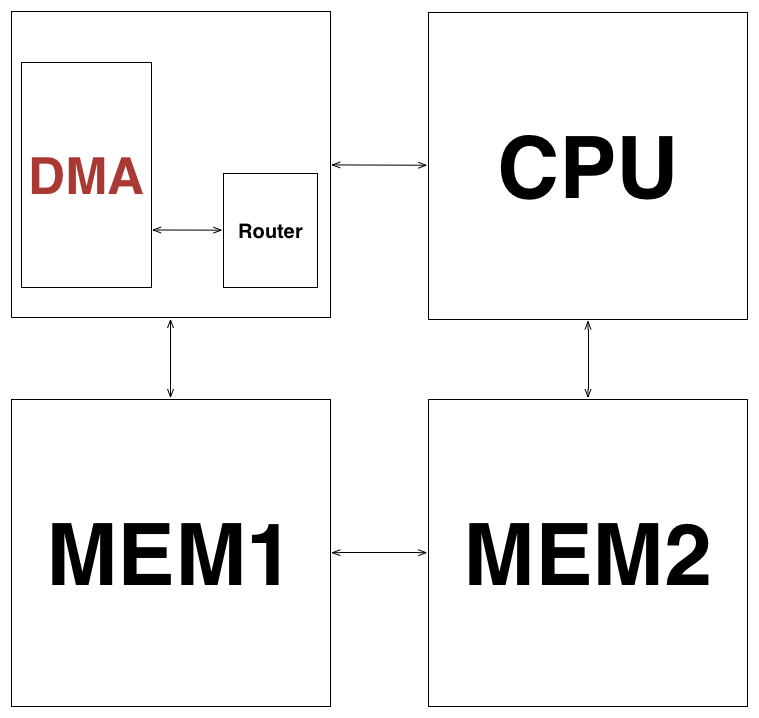
\includegraphics[width=0.8\textwidth]{Figures/DMA/DMATile}
    \caption{DMA module implemented as a shared DMA Controller tile}
    \label{fig:DMATile}
\end{figure}

\begin{figure}[h!]
    \centering
    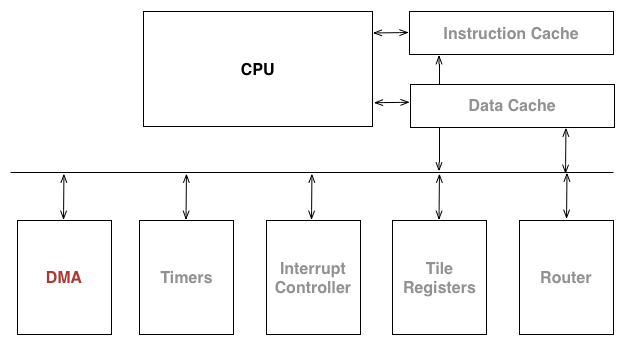
\includegraphics[width=0.8\textwidth]{Figures/DMA/Accelerator}
    \caption{DMA module Implemented as accelerator on an existing tile, on bottom left. Based upon figure from \cite{shmac-plan}}
    \label{fig:DMAAccelerator}
\end{figure}

There are different reasons for and against each option:
\begin{itemize}
    \item A full tile gives the benefit of having a full tile for the DMA implementation.
    This is useful for complex implementations that require much space.
    On the other hand, the smaller and more simple implementation, the less benefit of the extra space.
    \item The DMA Controller may also be implemented as an acceleratoron an already designed tile, such as a CPU, or a scratchpad memory.
    Since a entire tile can be partially powered down, a DMA module may very well be implemented without any significant cost in terms of power usage.
    In fact, a DMA module may work as the only active part of a tile as well.
    A tile with a DMA module can also use the DMA to transfer data between internal modules on the tile.
    However, this also means the DMA has to share the internal shared bus network with other modules.
\end{itemize}

For a basic implementation of a DMA in SHMAC, all that is needed for the DMA module to work is that it can transfer data from one address to another.
It does not need to know where in the system it is, and what route the data must take from the load address to the store address.
Figure \ref{fig:DMASHMAC1} shows an example where the DMA is implemented on a seperate tile.

\begin{figure}[h!]
    \centering
    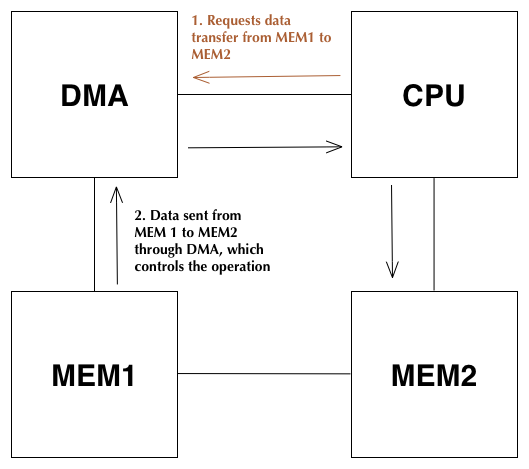
\includegraphics[width=0.7\textwidth]{Figures/DMA/DMASHMAC1}
    \caption{DMA module implemented as a tile on SHMAC, with basic transfer from MEM1 to MEM2 through itself}
    \label{fig:DMASHMAC1}
\end{figure}
 
As can be seen in the figure, the DMA tile recieves a request from its neighbouring CPU tile, and transfers data  from tile MEM1 to tile MEM2.
This would also work the same way if the DMA module was implemented on the CPU tile as an accelerator instead.
While this completes the basic goal of moving data on behalf of the CPU tile, it does not know or care where in the SHMAC system it is.
If two memory tiles are close to each other, while the active DMA tile is far away (for instance on the other side of the entire SHMAC board), the data would have to travel unnecessarily far to reach the goal, and the operation will slow down.

\begin{figure}[h!]
    \centering
    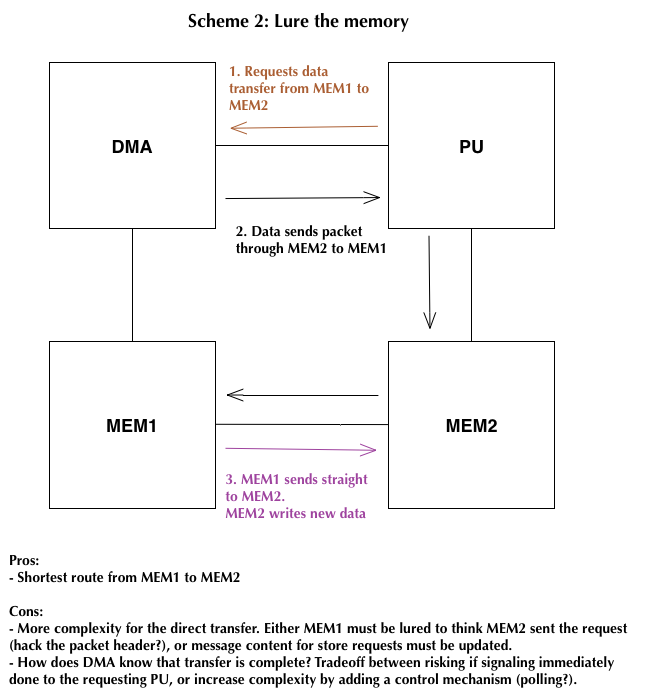
\includegraphics[width=0.7\textwidth]{Figures/DMA/DMASHMAC2}
    \caption{DMA implemented by tricking MEM1 to transfer data to MEM2}
    \label{fig:DMASHMAC2}
\end{figure}

Figure \ref{fig:DMASHMAC2} shows an implementation where the DMA tile sets up a transfer between MEM1 and MEM2, by tricking MEM1 to believe that the request source is MEM2, not the DMA module.
This could be done by sending a request signal through MEM2 to MEM1 with packet info claiming that the requestor is MEM2.
For this to work, both MEM1 and MEM2 need the sufficient hardware to perform load and store operations themselves.
This way, the distance is as short as possible, but how does the DMA tile know when the transfer is done, considering that it is not control the transfer itself?
It could ignore this part of the task, and signal the CPU that the transfer is complete as soon as the tricking request has been sent out, but depending on the storing tile (a memory tile, or another accelerator tile), the CPU will risk loading old data that has not yet been overwritten, should it load from the ''wrong'' address before new data has arrived.
Alternatively, the DMA module may be implemented with polling, so that it polls the MEM2 tile to see when the data transfer is complete.
This leads to additional complexity in implementing the DMA.
 
\begin{figure}[h!]
    \centering
    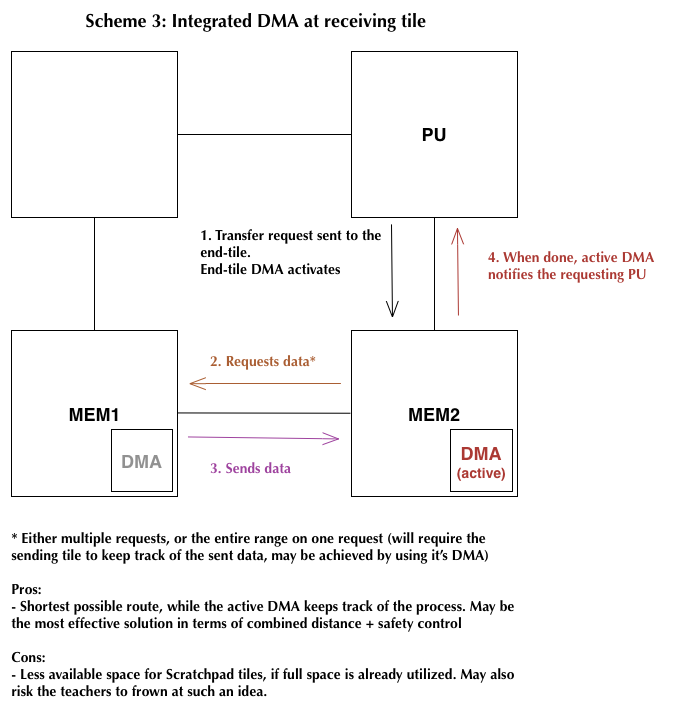
\includegraphics[width=0.8\textwidth]{Figures/DMA/DMASHMAC3}
    \caption{DMA module implemented directly on storing memory tile}
    \label{fig:DMASHMAC3}
\end{figure}
 
Figure \ref{fig:DMASHMAC3} shows an implementation where the DMA module has been implemented on the memory tiles themselves.
In this implementation, the CPU sends the DMA transfer request to the DMA on the storing tile.
As soon as the request reaches the DMA module on MEM2, it will generate load requests to MEM1.
As soon as data arrives, the DMA module will store the data in the store addresses, and signal the requesting CPU when the task is done.
The distance between MEM1 and MEM2 is kept as short as possible, and the DMA module keeps the transfer safe since it knows when the task is complete before signaling the CPU.
A drawback is that by implementing the DMA module directly on the memory tile, there will be less potential room for the memory size itself.

The DMA module and the entire transfer operation will also be more complex, since location now matters.
The DMA Controller must know where its own tile is located in the SHMAC system, before either passing on the request to the DMA Controller on the correct tile.
Alternatively the requesting CPU itself must know where the correct DMA module is (either by checking a look-up table, or deducing it from the destination address).

This alternative is more complex than the other two discussed, but if successfully implemented, it will save transfer time by making the distance between source and destination as short as possible, and the local DMA Controller on the receiving tile has full control of wheter the transfer is done or not.
This makes this alternative likely the one with best performance, and also most efficient if the distance it saves makes up for the more complex hardware required.

%In the first case, the DMA module must be implemented with knowledge of its own position, and with the ability to pass on requests to the correct module.
%This itself increases the complexity of the module.\todo{But also add favorable reasons?} 
%Another question also arises: would the DMA module in MEM2 send multiple single load requests to MEM1, or should it cooperate with the DMA module on MEM1 by sending only the start address and the transfer length, and letting the module on MEM1 load and send out the data?
%The latter case would be more efficient in terms of data transport, as only one request from MEM2 to MEM1 would be necessary, but at the same time, implementing a cooperation scheme between two DMA modules would further increase the complexity of the implementation.
%On a memory tile, further complexity also means less memory space.
%In summary, this is a compromise between memory size and efficiency.

\subsection{Other issues regarding use of DMA}

When implementing a DMA module, there are issues regarding its cooperation with the system that must be handled.
Among these are cache coherency and virtual memory.
These will be outside the scope of this project, but are relevant if a DMA module is to be implemented on SHMAC.

\subsubsection{Cache coherency}
Data that the DMA module is tranfering may also exist on the cache of a CPU \cite[p~594-595]{computer-construction}.
The DMA Controller only sees the data in the memory, and if the memory is overwritten, there will be different values in the cache and in the memory.
This is the cache coherency problem.
A way to deal with this is to invalidate the entry in the cache, and have the CPU reload data from the memory.
% SHMAC currently avoids the coherency problem for multiple cores by having shared data in uncachable memory, but since this will reduce performance due to the memory-gap, it is likely that SHMAC in the future will implement a different solution on this.

\subsubsection{Virtual memory}
If the system has virtual memory, a problem is whether the DMA module should work with virtual or physical addresses \cite[p~595]{computer-construction}.
The drawback with virtual addressing every address must be translated to physical addresses.
But the problem with physical addresses is that the transfer cannot easily cross a page boundry.
Contiguous data in the physical space is not necessarily contiguous in virtual memory.
When using physical addressing, DMA transfers must be constrained within same memory page.

\todo{Consider moving this entire paragraph to "future work"}
A possible solution may be to make the DMA work on virtual addresses, by providing the DMA module with with a small number of map entries that provide virtual-to-physical mapping for a transfer.
Another solution is for the operating system to break the DMA transfer into a series of transfers, each confined within a single physical page.
The transfers are then chained together and handled by an intelligent DMA unit that executes the series of transfers. 
For any of the solutions, the operating system must cooperate by not remapping the pages with a DMA transfer involving that page is in progress.

SHMAC does currently not implement virtual memory, but it is listed as a future task \cite[p~10]{shmac-plan}.
Therefore, this will be a future issue that needs to be solved if both DMA and virtual memory are to be used in SHMAC. 

\subsubsection{Multiple DMA requests operating on the same data field}
\todo{YUP!}
Yaman mentioned this. Write something sensible if time, or just wipe this out.


% - Cache coherency is not an issue when there is no cache :-) -K.
% 
% - Disagree: There are caches on SHMAC. Reread the planning paper!



% - Virtual memory is handled internally in the processors, the DMA operates only on physical addresses unless an IOMMU is used. -K.
%
% - Disagree. It is still a problem because virtual addresses and it's physical versions may not be aligned in memory. See what I have written.

%\subsection{Other options to consider}
%What is the data size? 
%Byte or bit? 
%Who can interrupt? 
%What type of interruptions may the DMA send out? 
%Multiple jobs?
%Generic DMA or specialized DMAs?
%
% - Commented out for the first draft. -K.
%
% - No time to write on this now 

